\chapter{Parte 3}
\label{cap:p3}

\section{Análise do problema}
Nesta 3ª parte do trabalho pretende-se introduzir o conceito do JIT
\emph{just-in-time}. O JIT preconiza a redução das folgas existentes entre
o fim de uma atividade e o início da atividade que a segue. 
As restrições de JIT podem ser generalizadas, para exprimir que o instante de
início da segunda operação deve acontecer num instante de tempo menor ou igual
do que o instante de fim da primeira operação.



\section{Ponto 1}

Considerando o gráfico inicial, pretende-se impor que a atividade 2 comece
imediatamente depois da atividade 1 ter começado, ou seja, $T_2 \le T_1 + D_1$
onde $T_2$ é o tempo da atividade 2, $T_1$ é o tempo da atividade 1 e $D_1$
a duração requerida para a atividade 1. Generalizando $T_j \le T_i + D_i$, onde
$T_j$ é o tempo da atividade j, $T_i$ é o tempo da atividade i e  e $D_1$
a duração requerida para a atividade i., tal que i precede j.

Com esta restrição, podemos achar o caminho mais longo até à atividade 2, para
calcular em seguida o tempo em que atividade 1 pode começar no instante mais
cedo, através da inequação anteriormente referida. Temos que, a duração no arco
da atividade 1 para atividade 2 é igual a 6, que a duração da atividade 1. Então
$T_2 \le T_1 + 6$

Como tal, o caminho mais longo para o nodo 2 é 6->7->4->2, onde as durações
somadas são $T_2 = 5 + 6 + 9 = 20$. Não se considera o tempo da atividade 2 pois esta
ainda não foi realizada. Para obter o valor do $T_1$, temos que $20 \le T_1
+ 6 \Leftrightarrow T_1 \ge 20 - 6 \Leftrightarrow T_1 \ge 14$. Com a restrição
de precedência da atividade 1 com a atividade 2 ($T_2 \ge T_1 + 6$) ficamos com 
$T_1 = 14$, que é o instante mais cedo que a atividade 1 pode começar.

\section{Ponto 2}

As atividades escolhidas do grafo gerado para este trabalho são as atividade
1 e 3. Então $T_3 \le T_1 + D_1 \Leftrightarrow T_3 \le T_1 + 6$. Acrescentou-se
esta restrição no modelo para resolução no \texttt{lp\_solve}, com o mesmo
\emph{output} apresentado na secção anterior, com o acréscimo desta restrição

\newpage

O \emph{output} produzido pelo \texttt{lp\_solve} é o seguinte:

\begin{verbatim}
Value of objective function: 26

Actual values of the variables:
Tfim                           26
T0                              0
Tini                            0
T1                             18
T3                             24
T5                             20
T4                             11
T7                              5
T10                             5
T6                              0
T9                             20
T11                            13

\end{verbatim}


O \emph{output} produzido pelo \texttt{lp\_solve} sem a restrição é o seguinte:

\begin{verbatim}
Value of objective function: 26

Actual values of the variables:
Tfim                           26
T0                              0
Tini                            0
T1                              4
T3                             24
T5                             20
T4                             11
T7                              5
T10                             5
T6                              0
T9                             20
T11                            13

\end{verbatim}

Come se pode ver a atividade 1, ao contrário do modelo do trabalho 1,
adiantou-se para poder cumprir a restrição.


\section{Ponto 3}

Como já foi anteriormente referido nas anteriores secções (Parte I --- descrição
das restrições e Parte II --- passagem das restrições para variáveis de decisão,
neste caso arcos, sendo o modelo primal baseado em nodos), a passagem de uma
restrição no modelo primal para dual passa de uma restrição para um arco, sendo
o arco em questão $X_{3~1}$, a partir da restrição mencionada anteriormente.

\section{Ficheiro de \emph{input} de \emph{Relax4}}


\begin{verbatim}
12                   
21                   
1    2     0     1 
1    6     0     1 
6    7    -5     1 
6   10    -5     1 
2    4    -4     1 
2    3    -4     1 
3    8    -6     1 
4    5    -9     1 
4    8    -9     1 
5    8    -4     1 
5   12    -4     1 
7    4    -6     1 
7    5    -6     1 
7    9    -6     1 
10   5    -8     1 
10  11    -8     1 
10   9    -8     1 
11   9    -7     1 
9   12    -2     1 
8   12    -2     1 
8    3    6      1 -> restrição JIT
1                 
0                    
0                    
0                    
0                    
0                    
0                    
0                    
0                    
0                    
0                    
-1                
\end{verbatim}


\newpage
\section{\emph{Output} produzido pelo \emph{Relax 4}}

\begin{verbatim}
END OF READING
 NUMBER OF NODES = 12, NUMBER OF ARCS = 21
 CONSTRUCT LINKED LISTS FOR THE PROBLEM
 CALLING RELAX4 TO SOLVE THE PROBLEM
 ***********************************
 TOTAL SOLUTION TIME =  0. SECS.
 TIME IN INITIALIZATION =  0. SECS.
   1 6  1.
   6 7  1.
   3 8  1.
   4 5  1.
   5 8  1.
   7 4  1.
   8 12  1.
   8 3  1.
 OPTIMAL COST =  -26.
 NUMBER OF AUCTION/SHORTEST PATH ITERATIONS = 55
 NUMBER OF ITERATIONS =  7
 NUMBER OF MULTINODE ITERATIONS =  1
 NUMBER OF MULTINODE ASCENT STEPS =  1
 NUMBER OF REGULAR AUGMENTATIONS =  1
 ***********************************

\end{verbatim}

\newpage
\section{Resultado}
\label{p3:resultado}


De acordo com o ficheiro de \emph{output} obtido, o caminho mais longo tem
a duração de 26 unidades de tempo (multiplicando por -1, devido ao uso do método
de simplex dual) e é o que passa pelas arestas $X_{ini\_6}$,
$X_{6\_7}$, $X_{7\_4}$, $X_{1\_3}$, $X_{3\_1}$ $X_{4\_5}$, $X_{5\_3}$ e $X_{3\_fim}$. Em termos
gráficos, o resultado é o apresentado na figura~\ref{p3:fig:caminho_critico}. As
setas de linha cheia indicam as arestas que fazem parte do caminho mais longo,
e os nós por onde esse caminho passa foram colocados a verde.

\begin{figure}[<+htpb+>]
	\centering
	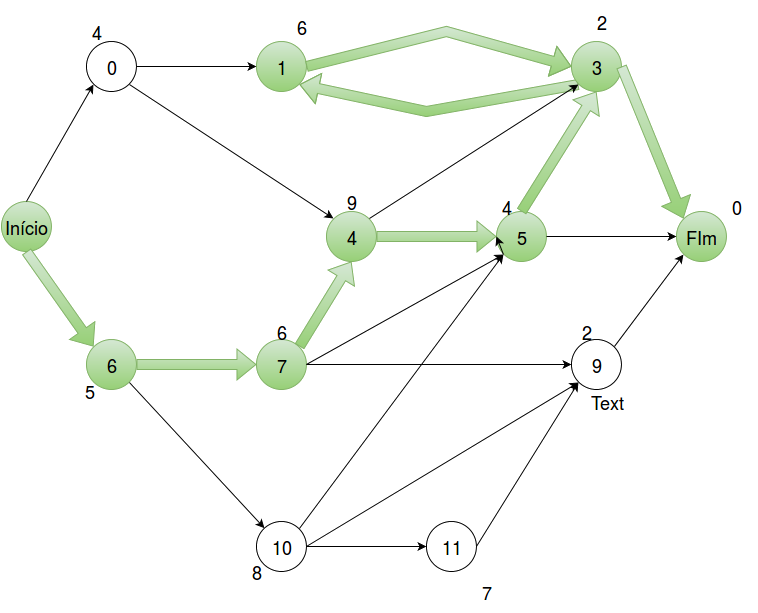
\includegraphics[scale=0.5]{./img/novo_critic}
	\caption{Novo caminho critico}
\label{p3:fig:caminho_critico}
\end{figure}
\section{Validação do modelo}

Para validar os resultados, tanto na função objetivo como nas restrições,
substituímos os valores das variáveis de decisão pelo valor que estas tomam na
solução que o \emph{Relax4} indica como ótima. A ideia é verificar que os valores
das variáveis de decisão obtidos confirmam o valor da função objetivo obedecendo
a todas as restrições.

\subsection{Variáveis de decisão}

No resultado obtido todas as variáveis são de facto binárias, tomam apenas
o valor de 0 ou 1, tal como esperado.


\subsection{Restrições}

\begin{itemize}

\item Nodo Inicio 

$1-X_{ini\_6} - X_{ini\_0} = 0$

$1 - 1 - 0 = 0$

\item Nodo 0 

$X_{ini\_0}-X_{0\_1}-X_{0\_4} = 0$

$0 - 0 - 0 = 0$

\item Nodo 1 


$	X_{0\_1}-X_{1\_3} + X_{3\_1} = 0$

$0 - 1 + 1 = 0$

\item Nodo 3 


$	X_{1\_3} + X_{4\_3} + X_{5\_3}-X_{3\_fim} - X_{3\_1} = 0$

$1 + 0 + 1 - 1 + 1 = 0$

\item Nodo 4 

$	X_{0\_4} + X_{7\_4} - X_{4\_3} - X_{4\_5} = 0$

$0 + 1 - 0 - 1= 0$

\item Nodo 5 

$X_{4\_5} + X_{7\_5} + X_{10\_5} - X_{5\_3} - X_{5\_fim} = 0$

$1 + 0 + 0 - 1 - 0 = 0$

\item Nodo 6 

$X_{ini\_6} - X_{6\_7} - X_{6\_10} = 0$

$1 - 1 - 0 = 0$

\item Nodo 7 

$X_{6\_7}- X_{7\_4}- X_{7\_5} - X_{7\_9} = 0$

$1 - 1 - 0 - 0 = 0$

\item Nodo 9 

$X_{7\_9} + X_{10\_9} + X_{11\_9} - X_{9\_fim} = 0$

$0 + 0 + 0 - 0 = 0$

\item Nodo 10 

$X_{6\_10} - X_{10\_5} - X_{10\_9} - X_{10\_11} = 0$

$0 - 0 - 0 - 0 = 0$

\item Nodo 11 

$X_{10\_11} - X_{11\_9} = 0$

$0 - 0 = 0$

\item Nodo Fim 

$X_{3\_fim} + X_{5\_fim} + X_{9\_fim} - 1 = 0$

$1 + 0 + 0 - 1 = 0$



\end{itemize}


Assim conclui-se que todas as restrições são respeitadas.
